\documentclass[conference,a4paper]{IEEEtran}
\IEEEoverridecommandlockouts

% ---------------------------------------------------------------------------
% Pacotes
% ---------------------------------------------------------------------------
\usepackage[utf8]{inputenc}
\usepackage[T1]{fontenc}
\usepackage[brazil]{babel}
\usepackage{mathptmx} % Times (texto e matemática), padrão IEEE
\usepackage{amsmath,amssymb,amsfonts}
\usepackage{bm}
\usepackage{graphicx}
\usepackage{booktabs}
\usepackage{multirow}
\usepackage{array}
\usepackage{xcolor}
\usepackage{cite}
\usepackage{url}
\usepackage[hidelinks]{hyperref}
\usepackage{microtype}

\graphicspath{{figures/}}
% parâmetros de posicionamento de floats (menos páginas só de figuras)
\renewcommand{\topfraction}{0.92}
\renewcommand{\bottomfraction}{0.6}
\renewcommand{\textfraction}{0.06}
\renewcommand{\floatpagefraction}{0.85}
\renewcommand{\dbltopfraction}{0.92}
\renewcommand{\dblfloatpagefraction}{0.85}
\setcounter{topnumber}{4}
\setcounter{dbltopnumber}{3}
\setcounter{totalnumber}{6}
\renewcommand{\arraystretch}{1.08}
\newcommand{\tabfont}{\footnotesize}
\def\UrlBreaks{\do\/\do-\do_\do.}

\hyphenation{SARIMAX Prophet Light-GBM Ran-dom Fo-rest dessa-zo-na-li-za-da}

\renewcommand{\IEEEkeywordsname}{Palavras-chave}
\begin{document}

\title{Previsão de Temperatura e de Chuva na Austrália:\\
Séries Temporais e Classificação Supervisionada\\ no Conjunto \textit{Rain in Australia}}

\author{\IEEEauthorblockN{João Pedro Dias de Carvalho}
\IEEEauthorblockA{Programa de Pós-Graduação em Ciências Computacionais e Modelagem Matemática (CompMat)\\
Universidade do Estado do Rio de Janeiro (UERJ)\\
Disciplina: Aprendizado de Máquina em Sistemas Dinâmicos --- Prof. Americo Cunha}}

\maketitle

% ===========================================================================
\begin{abstract}
Este trabalho aplica técnicas de regressão e de classificação a dados
meteorológicos reais: cerca de 145 mil observações diárias de 49 estações australianas
(2007--2017), disponíveis no Kaggle. Na regressão, previ a temperatura máxima média semanal
de Sydney com quatro modelos supervisionados de séries temporais: SARIMAX com harmônicos de
Fourier e erros ARMA, Prophet, decomposição STL seguida de ARIMA e a média simples dos três.
Os hiperparâmetros foram escolhidos por AIC ou validação e os modelos foram avaliados em
78 semanas futuras, em previsão de longo prazo e de um passo à frente, além de um
\textit{backtest} com origem móvel. O SARIMAX obteve o menor erro (RMSE de 1,65\,°C no longo
prazo e 1,59\,°C um passo à frente, 22\% abaixo do modelo ingênuo) e resíduos sem autocorrelação
detectável, mas o teste de Diebold--Mariano não o distingue do Prophet nem da combinação.
Na classificação, previ se choveria no dia seguinte (22\% de dias positivos) com regressão
logística (um GLM), KNN, Random Forest e LightGBM, após engenharia de atributos que inclui
codificação circular do vento, tendência barométrica e indicadores de ausência. Com validação
cruzada estratificada, limiar escolhido fora da amostra e teste temporal em 2016--2017, o
LightGBM foi o melhor (ROC-AUC de 0,889, PR-AUC de 0,752 e F1 de 0,674), seguido pela Random
Forest. A umidade às 15h, a rajada de vento e a variação da pressão foram as variáveis mais
informativas. Discuto as premissas dos modelos, a calibração das probabilidades e as
limitações para uso operacional.
\end{abstract}

\begin{IEEEkeywords}
séries temporais, SARIMAX, Prophet, STL, combinação de previsões, classificação desbalanceada,
regressão logística, gradient boosting, meteorologia.
\end{IEEEkeywords}

% ===========================================================================
\section{Introdução e contextualização}

Prever o tempo é um problema clássico de sistemas dinâmicos: a atmosfera evolui segundo
equações não lineares e sensíveis às condições iniciais~\cite{lorenz1963deterministic}, e as observações em superfície (temperatura, pressão, umidade, vento)
são projeções ruidosas e parciais desse estado. Ainda assim, padrões estatísticos robustos,
como o ciclo anual de temperatura ou a queda de pressão que antecede frentes frias, permitem
construir previsores úteis, baseados em dados, para agricultura, energia, defesa civil e saúde
pública. A temperatura semanal, por exemplo, orienta o planejamento da demanda de energia e de
alertas de calor, e a probabilidade de chuva no dia seguinte afeta a logística e o manejo de recursos hídricos.

Este trabalho usa o conjunto \textit{Rain in Australia}~\cite{kaggle_weatheraus}, derivado das
observações diárias do \textit{Bureau of Meteorology} (BoM) australiano~\cite{bom_climate}
e originalmente distribuído com o pacote \textit{rattle}~\cite{williams2011rattle}. Cada
registro corresponde a um par (estação, dia) e contém 19 variáveis meteorológicas (16 numéricas e 3 direções de vento), além da
indicação de chuva no próprio dia (\texttt{RainToday}) e no dia seguinte (\texttt{RainTomorrow}). Formulei dois problemas:
\begin{enumerate}
\item \textbf{Regressão (série temporal):} prever a temperatura máxima média semanal de Sydney,
com horizontes de uma a 78 semanas;
\item \textbf{Classificação (binária):} prever se choverá mais de 1\,mm nas 24\,h que terminam às 9h do dia seguinte
(\texttt{RainTomorrow}) em qualquer uma das 49 estações.
\end{enumerate}
O restante do texto descreve os dados e o pré-processamento (Seção~\ref{sec:metodo}), a
formulação dos modelos, os experimentos (Seção~\ref{sec:exp}) e a discussão (Seção~\ref{sec:disc}).
O código (Python) e um \textit{notebook} executável acompanham este relatório.

% ===========================================================================
\section{Metodologia e dados}\label{sec:metodo}

\subsection{Descrição do conjunto de dados}
A base tem 145.460 linhas e 23 colunas (16 numéricas, 6 categóricas e a data), de 01/11/2007
a 25/06/2017. A Tabela~\ref{tab:descritiva} resume as variáveis numéricas. Cerca de 10,3\% das
células estão vazias e só 38,8\% das linhas são completas.

\begin{table}[!t]
\centering
\caption{Estatísticas descritivas das variáveis numéricas (base completa).}
\label{tab:descritiva}
\tabfont
\resizebox{\columnwidth}{!}{\begin{tabular}{lrrrrrrr}
\toprule
 & Média & DP & Mín & Mediana & Máx & Assimetria & Faltantes (\%) \\
\midrule
MinTemp & 12,2 & 6,4 & $-$8,5 & 12,0 & 33,9 & 0,0 & 1,0 \\
MaxTemp & 23,2 & 7,1 & $-$4,8 & 22,6 & 48,1 & 0,2 & 0,9 \\
Rainfall & 2,4 & 8,5 & 0,0 & 0,0 & 371,0 & 9,8 & 2,2 \\
Evaporation & 5,5 & 4,2 & 0,0 & 4,8 & 145,0 & 3,8 & 43,2 \\
Sunshine & 7,6 & 3,8 & 0,0 & 8,4 & 14,5 & $-$0,5 & 48,0 \\
WindGustSpeed & 40,0 & 13,6 & 6,0 & 39,0 & 135,0 & 0,9 & 7,1 \\
WindSpeed9am & 14,0 & 8,9 & 0,0 & 13,0 & 130,0 & 0,8 & 1,2 \\
WindSpeed3pm & 18,7 & 8,8 & 0,0 & 19,0 & 87,0 & 0,6 & 2,1 \\
Humidity9am & 68,9 & 19,0 & 0,0 & 70,0 & 100,0 & $-$0,5 & 1,8 \\
Humidity3pm & 51,5 & 20,8 & 0,0 & 52,0 & 100,0 & 0,0 & 3,1 \\
Pressure9am & 1017,6 & 7,1 & 980,5 & 1017,6 & 1041,0 & $-$0,1 & 10,4 \\
Pressure3pm & 1015,3 & 7,0 & 977,1 & 1015,2 & 1039,6 & $-$0,0 & 10,3 \\
Cloud9am & 4,4 & 2,9 & 0,0 & 5,0 & 9,0 & $-$0,2 & 38,4 \\
Cloud3pm & 4,5 & 2,7 & 0,0 & 5,0 & 9,0 & $-$0,2 & 40,8 \\
Temp9am & 17,0 & 6,5 & $-$7,2 & 16,7 & 40,2 & 0,1 & 1,2 \\
Temp3pm & 21,7 & 6,9 & $-$5,4 & 21,1 & 46,7 & 0,2 & 2,5 \\
\bottomrule
\end{tabular}
}
\end{table}

\subsection{Análise exploratória e pré-processamento}

\textbf{Dados ausentes.} A Fig.~\ref{fig:missing} mostra que a ausência é, em grande parte,
\emph{estrutural}: 19 estações nunca mediram insolação (\texttt{Sunshine}) e 16 nunca mediram
evaporação. Como a ausência não é aleatória, descartar linhas eliminaria 61\% dos dados e
introduziria viés geográfico. Por isso, imputei a mediana \emph{dentro} do
\textit{pipeline} de validação, o que evita vazamento de informação, e acrescentei indicadores
binários de ausência. Removi apenas as 3.267 linhas (2,2\%) sem o alvo.

\begin{figure*}[!t]
\centering
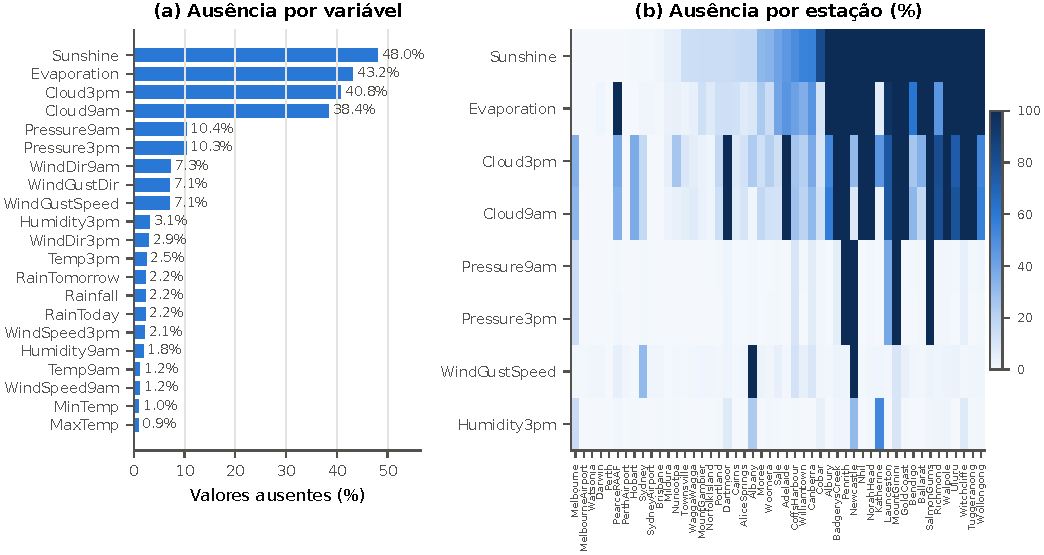
\includegraphics[width=\textwidth]{eda_missing.pdf}
\caption{Valores ausentes. (a) Percentual por variável. (b) Percentual por estação para as
variáveis mais afetadas: as faixas escuras (100\%) indicam estações sem o instrumento, ou seja,
ausência estrutural, não aleatória.}
\label{fig:missing}
\end{figure*}

\textbf{Inconsistências.} Verifiquei regras físicas e lógicas: duplicatas (estação, dia),
$T_{\min} > T_{\max}$, umidade fora de $[0,100]$, chuva negativa, coerência entre
\texttt{RainToday} e $\texttt{Rainfall} > 1$\,mm e a identidade
$\texttt{RainTomorrow}(t) = \texttt{RainToday}(t+1)$. Todas foram satisfeitas, exceto três
registros de nebulosidade igual a 9, código de ``céu obstruído'' e não uma medida em oitavos,
que foram convertidos em ausentes. A última identidade confirma a definição do alvo e reforça
que nenhuma informação de $t+1$ pode entrar como preditor. Há, porém, uma sobreposição temporal
própria do conjunto: \texttt{RainToday} mede a chuva nas 24\,h até as 9h~\cite{williams2011rattle},
de modo que o alvo cobre o intervalo das 9h de $t$ às 9h de $t+1$. As medições das 15h
(\texttt{Humidity3pm}, \texttt{Pressure3pm}, \texttt{Cloud3pm}, \texttt{Temp3pm}) e a rajada
máxima até a meia-noite (\texttt{WindGustSpeed}) caem dentro dessa janela. Não há vazamento, pois
esses valores já são conhecidos ao fim do dia $t$, mas o horizonte efetivo da previsão é de cerca
de 9 a 18\,h, e parte da tarefa é de \textit{nowcasting}. Há ainda 4.112 dias de calendário
sem registro em algumas estações, o que foi levado em conta ao construir variáveis defasadas.

\textbf{Distribuições e \textit{outliers}.} \texttt{Rainfall} (assimetria de 9,8) e
\texttt{Evaporation} (3,8) têm caudas longas à direita. Pela regra de Tukey
(1,5$\times$IQR)~\cite{tukey1977eda}, 18\% dos dias têm chuva ``atípica'', porque o primeiro
quartil e a mediana são zero e o IQR é minúsculo. Esses extremos são eventos reais, justamente os de interesse, e não erros. Por
isso, não os removi: apliquei $\log(1+x)$ e preferi modelos robustos (árvores) ou
padronizados (z-score). Os histogramas de todas as variáveis estão no \textit{notebook}.


\textbf{Correlação e alvo.} Há blocos fortemente colineares, como
\texttt{Pressure9am}--\texttt{Pressure3pm} ($r=0{,}96$) e \texttt{MaxTemp}--\texttt{Temp3pm}
($r=0{,}98$) (Fig.~\ref{fig:corr}). O alvo é desbalanceado (22,4\% de ``Sim'', razão de
3,5:1) e varia muito entre estações, de 7\% em Woomera, no deserto, a 37\% em Portland, e
entre meses, com pico no inverno austral (Fig.~\ref{fig:alvo}).

\begin{figure}[!t]
\centering
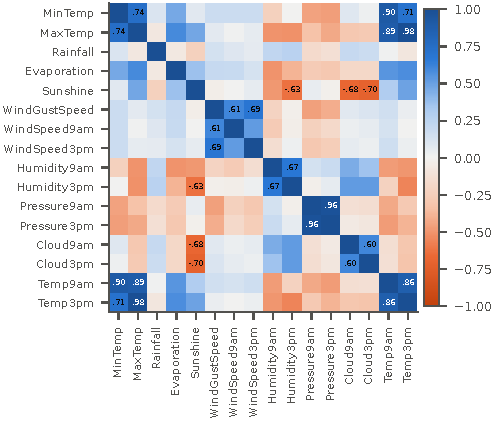
\includegraphics[width=\columnwidth]{eda_correlacao.pdf}
\caption{Matriz de correlação de Pearson; valores com $|r|\ge 0{,}6$ estão anotados.}
\label{fig:corr}
\end{figure}

\begin{figure*}[!t]
\centering
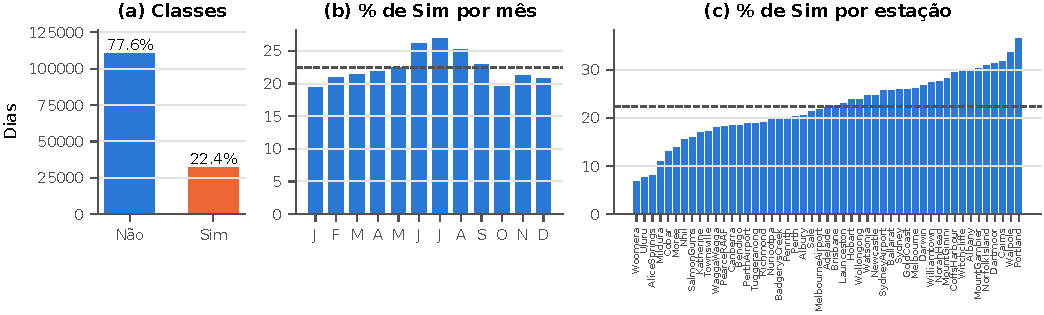
\includegraphics[width=\textwidth]{eda_alvo_classificacao.pdf}
\caption{Alvo da classificação. (a) Frequência das classes. (b) Proporção de dias seguidos de
chuva por mês. (c) Proporção por estação. A linha tracejada é a média global (22,4\%).}
\label{fig:alvo}
\end{figure*}

\textbf{Engenharia de atributos (classificação).} A partir das variáveis brutas, criei 41
preditores, todos calculados apenas com informação disponível até o dia $t$:
\begin{itemize}
\item \emph{transformações:} $\log(1+x)$ da chuva e da evaporação;
\item \emph{dinâmica intradiária:} amplitude térmica e diferenças 15h$-$9h de temperatura,
pressão, umidade e nebulosidade;
\item \emph{dinâmica de 24\,h:} variação de pressão (tendência barométrica), de umidade e de
temperatura em relação ao dia anterior na mesma estação, além de \texttt{RainYesterday};
\item \emph{direções do vento} (16 pontos) como variáveis circulares
$(\sin\theta,\cos\theta)$, de modo que N e NNO fiquem próximos;
\item \emph{sazonalidade:} $\sin$ e $\cos$ de $2\pi\,\text{dia}/365{,}25$;
\item \emph{indicadores de ausência} para insolação, evaporação, nebulosidade, pressão e rajada;
\item \emph{estação:} \textit{target encoding}~\cite{micci2001target} com ajuste cruzado
(\textit{cross-fitting}), que substitui 49 categorias pela taxa de chuva suavizada da estação.
\end{itemize}
Depois disso, as variáveis numéricas são imputadas pela mediana e padronizadas.

\textbf{Série da regressão.} Para Sydney, reindexei o calendário diário, que tem 91 dias
sem \texttt{MaxTemp}, e calculei a média semanal (semanas terminadas no domingo), exigindo
pelo menos 4 dias válidos. As 12 semanas que não atingem esse mínimo (2,4\% da série) foram
interpoladas linearmente. A agregação semanal filtra o ruído da escala sinótica (alguns dias), praticamente
imprevisível com semanas de antecedência, e realça a dinâmica sazonal. O resultado são 490
semanas (fev/2008 a jun/2017; Fig.~\ref{fig:serie}).

\begin{figure*}[!t]
\centering
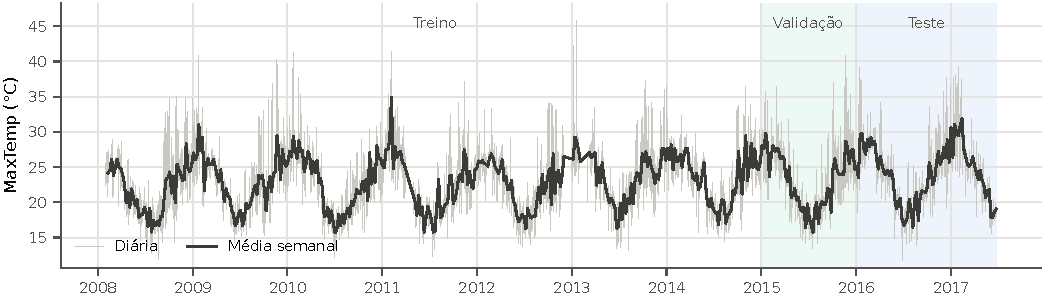
\includegraphics[width=\textwidth]{reg_serie.pdf}
\caption{Temperatura máxima em Sydney: série diária (cinza claro) e média semanal (preto).
As faixas indicam os períodos de validação (2015) e de teste (jan/2016 a jun/2017).}
\label{fig:serie}
\end{figure*}

Na série original, o teste ADF~\cite{dickey1979adf} rejeita a raiz unitária e o
KPSS~\cite{kwiatkowski1992kpss} não rejeita a estacionariedade (Tabela~\ref{tab:estac}), o que
indica $d=0$. Na série dessazonalizada, o ADF continua rejeitando a raiz unitária, mas o KPSS de
nível rejeita a estacionariedade. Esse conflito é típico de uma série estacionária em torno de
uma tendência, o que se confirma com o KPSS com tendência, que não rejeita a estacionariedade
($p\ge0{,}10$). Isso aponta uma variação lenta de nível e motiva testar um termo de tendência
determinística. A decomposição STL (Fig.~\ref{fig:stl}) mostra
sazonalidade dominante, com força $F_S = \max\{0,\,1-\mathrm{Var}(R)/\mathrm{Var}(S+R)\}
\approx 0{,}81$~\cite{wang2006characteristic,hyndman2021fpp3}, e tendência fraca ($F_T\approx 0{,}09$).

\begin{table}[!t]
\centering
\caption{Testes de estacionariedade (treino e validação, 2008--2015). Os p-valores do KPSS são
limitados à faixa da tabela de interpolação: 0,100 significa $p\ge0{,}10$ e 0,010, $p\le0{,}01$.
KPSS: estacionariedade em nível; KPSS-ct: estacionariedade em torno de tendência linear.}
\label{tab:estac}
\tabfont
\resizebox{\columnwidth}{!}{\begin{tabular}{lrrrrrr}
\toprule
 & ADF estat. & ADF p-valor & KPSS estat. & KPSS p-valor & KPSS-ct estat. & KPSS-ct p-valor \\
\midrule
Série original & $-$7,451 & 0,000 & 0,074 & 0,100 & 0,022 & 0,100 \\
Dessazonalizada (STL) & $-$11,132 & 0,000 & 1,026 & 0,010 & 0,117 & 0,100 \\
\bottomrule
\end{tabular}
}
\end{table}

\begin{figure}[!t]
\centering
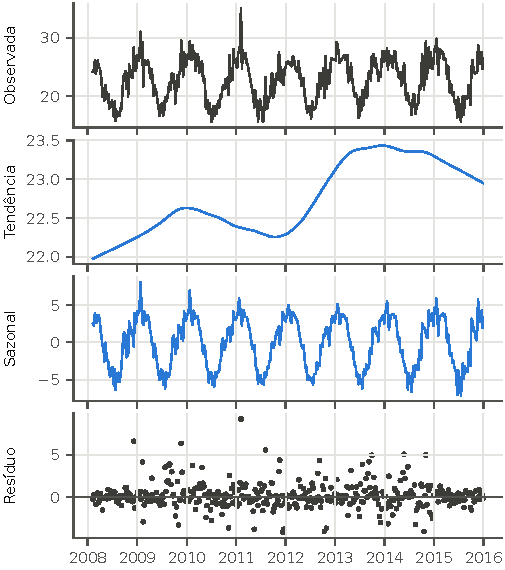
\includegraphics[width=\columnwidth]{reg_stl.pdf}\\[2pt]
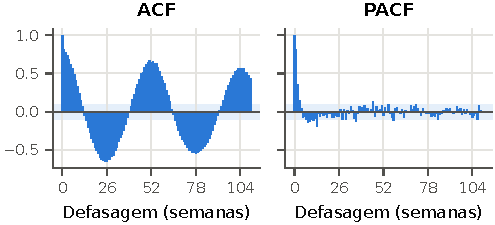
\includegraphics[width=\columnwidth]{reg_acf.pdf}
\caption{Acima: decomposição STL robusta da série semanal (2008--2015). Abaixo: ACF e PACF da
série semanal original, com banda de 95\% sob ruído branco; a oscilação com período de 52 semanas reflete a
sazonalidade determinística.}
\label{fig:stl}
\end{figure}

\subsection{Modelos de regressão}

Os quatro modelos são supervisionados: aprendem, a partir de pares (passado, futuro), uma
função $\hat y_{t+h} = f(y_{1:t}, t)$. Seja $m = 365{,}25/7 \approx 52{,}18$ o período
anual em semanas.

\textbf{(1) SARIMAX com regressão harmônica.} Com $m\approx 52$, o polinômio sazonal
$(P,D,Q)_{52}$ do SARIMA é caro e instável. Por isso, usei o \textbf{X} do
SARIMAX~\cite{box2015time,hyndman2021fpp3}: $K$ pares de Fourier como regressores exógenos e
erros ARMA$(p,q)$:
\begin{equation}
y_t = \beta_0 + \beta_1 t + \sum_{k=1}^{K}\!\Big[a_k\sin\tfrac{2\pi k t}{m} + b_k\cos\tfrac{2\pi k t}{m}\Big] + \eta_t,
\label{eq:sarimax}
\end{equation}
com $\phi(B)\eta_t = \theta(B)\varepsilon_t$ e $\varepsilon_t \sim \mathcal N(0,\sigma^2)$. Os
parâmetros são estimados por máxima verossimilhança exata via filtro de
Kalman~\cite{durbin2012time,seabold2010statsmodels}. Como não há polinômio sazonal, o modelo é,
a rigor, uma regressão harmônica com erros ARMA; o nome SARIMAX vem da classe do statsmodels
usada no ajuste.

\textbf{(2) Prophet.} Modelo aditivo bayesiano~\cite{taylor2018prophet}:
$y(t) = g(t) + s(t) + \varepsilon_t$, em que $g$ é uma tendência linear por partes, com pontos
de mudança sob \textit{prior} de Laplace de escala $\tau$, e
$s(t) = \sum_{n=1}^{N}[a_n\cos(2\pi n t/365{,}25) + b_n\sin(2\pi n t/365{,}25)]$, com $t$ em dias e
\textit{prior} normal de escala $\sigma_s$. A estimação é por MAP no Stan~\cite{carpenter2017stan}.

\textbf{(3) Decomposição STL + ARIMA.} A STL robusta~\cite{cleveland1990stl} separa
$y_t = T_t + S_t + R_t$ por suavizações LOESS iterativas. Como cada semana do ano tem só
cerca de 7 observações no treino, o perfil sazonal $\hat S(c)$, com $c = t \bmod 52$, é a média
de $S_t$ por posição, suavizada circularmente entre semanas vizinhas. A série dessazonalizada
$a_t = y_t - \hat S(t \bmod 52)$ é modelada por um ARIMA, e a previsão é
$\hat y_{t+h} = \hat a_{t+h} + \hat S((t+h)\bmod 52)$.

\textbf{(4) Combinação.} Média simples das três previsões,
$\hat y^{\mathrm{comb}}_t = \frac13(\hat y^{\mathrm{SARIMAX}}_t+\hat y^{\mathrm{Prophet}}_t+\hat y^{\mathrm{STL}}_t)$.
Com erros de média zero, seu erro quadrático médio é
$\frac{1}{9}\sum_{i,j}\rho_{ij}\sigma_i\sigma_j$, que nunca supera o do pior componente e é
menor que o de todos quando os erros têm variâncias parecidas e são pouco
correlacionados~\cite{bates1969combination}. Por não estimar pesos, a combinação não sobreajusta.
O intervalo de 95\% foi aproximado pela média dos limites dos componentes, aproximação
conservadora quando $\rho_{ij}<1$, pois ignora a redução de variância da média.

\subsection{Modelos de classificação}

\textbf{Regressão logística} --- um GLM com distribuição de Bernoulli e ligação
logit~\cite{nelder1972glm}: $\Pr(Y=1\mid\mathbf x) = \sigma(\beta_0+\bm\beta^\top\mathbf x)$.
Os coeficientes minimizam a log-verossimilhança negativa ponderada com penalidade L2,
\begin{equation}
\min_{\bm\beta}\; -\sum_i w_{y_i}\big[y_i\log p_i+(1-y_i)\log(1-p_i)\big] + \tfrac{1}{2C}\lVert\bm\beta\rVert_2^2,
\end{equation}
com pesos $w_c = n/(2n_c)$ que compensam o desbalanceamento. O termo $e^{\beta_j}$ é a razão
de chances associada a um desvio-padrão do preditor $j$.

\textbf{KNN}~\cite{cover1967knn,dudani1976distance}: $\hat p(\mathbf x) = \sum_{i\in N_k(\mathbf x)} w_i y_i/\sum w_i$,
com $w_i = 1/\lVert\mathbf x-\mathbf x_i\rVert_2$. É não paramétrico, com fronteira local e flexível.

\textbf{Random Forest}~\cite{breiman2001rf}: média de $B$ árvores, cada uma treinada em uma
amostra \textit{bootstrap} e com sorteio de variáveis em cada nó, o que reduz a correlação
entre árvores e, portanto, a variância.

\textbf{LightGBM}~\cite{ke2017lightgbm,friedman2001gbm,chen2016xgboost}: modelo aditivo
$F_M(\mathbf x) = \sum_{j=1}^{M}\eta f_j(\mathbf x)$, em que cada árvore $f_j$ é ajustada por um
passo de Newton, com o gradiente e a hessiana da perda logística avaliados em $F_{j-1}$, com crescimento \textit{leaf-wise}, histogramas e
regularização L2.

A escolha cobre um modelo linear interpretável (um GLM), um modelo
baseado em distância e dois \textit{ensembles} de árvores, aptos a capturar interações não
lineares entre umidade, pressão e vento.

% ===========================================================================
\section{Experimentos e resultados}\label{sec:exp}

Toda a implementação foi feita em Python, com pandas~\cite{mckinney2010pandas},
NumPy~\cite{harris2020numpy}, SciPy~\cite{virtanen2020scipy},
statsmodels~\cite{seabold2010statsmodels}, Prophet~\cite{taylor2018prophet},
scikit-learn~\cite{pedregosa2011sklearn}, LightGBM~\cite{ke2017lightgbm} e
Matplotlib~\cite{hunter2007matplotlib}, com semente fixa (42).

\subsection{Configuração da regressão}
A divisão é estritamente temporal: treino de fev/2008 a dez/2014 (360 semanas), validação em
2015 (52) e teste de jan/2016 a jun/2017 (78). Os hiperparâmetros foram escolhidos em grade:
\begin{itemize}
\item \emph{SARIMAX:} $K\in\{1,2,3,4,6\}$, $p,q\in\{0,1,2\}$, tendência constante ou linear
(90 modelos), selecionados pelo AIC~\cite{akaike1974new}, critério baseado na verossimilhança
das inovações um passo à frente;
\item \emph{Prophet:} $N\in\{3,5,10\}$, $\tau\in\{0{,}001;0{,}01;0{,}1;0{,}5\}$,
$\sigma_s\in\{1,10\}$, selecionados pelo RMSE na validação;
\item \emph{STL:} janela sazonal $\in\{7,13,25,53\}$, suavização $\in\{1,3,5,9\}$ e seis
especificações ARIMA, selecionadas pelo RMSE na validação.
\end{itemize}
Os modelos escolhidos (Tabela~\ref{tab:hp_reg}) foram retreinados em 2008--2015 e avaliados
em dois cenários: \textbf{(A) longo prazo}, com uma única previsão para $h=1,\dots,78$ semanas;
e \textbf{(B) um passo à frente}, em que, a cada semana do teste, previ a seguinte com todas
as observações já disponíveis. No cenário B, SARIMAX e STL mantêm os parâmetros e atualizam o
estado pelo filtro de Kalman; o Prophet, que não tem estado dinâmico, é retreinado toda semana.
As referências mínimas são o ingênuo sazonal, $\hat y_{t+h}=y_{t+h-52}$, no cenário A e a
persistência, $\hat y_{t+1}=y_t$, no cenário B. Por fim, um \textit{backtest} com origem móvel
treina até o fim de 2011, 2012, 2013 e 2014 e prevê o ano seguinte inteiro ($h=52$), sem usar
o período de teste. Como 2015 também serviu para escolher os hiperparâmetros, o RMSE desse
ano no \textit{backtest} é levemente otimista.

\begin{table*}[!t]
\centering
\caption{Hiperparâmetros escolhidos e RMSE (°C) na validação (2015), com os modelos treinados até 2014.}
\label{tab:hp_reg}
\tabfont
\begin{tabular}{llr}
\toprule
 & Configuração & RMSE val \\
\midrule
SARIMAX & ARMA(1,1) + Fourier K=2, tendência=ct & 1,63 \\
Prophet & Fourier anual N=3, tau=0.001, sigma\_s=10.0 & 1,54 \\
STL & STL(janela=53), suav.=3 + ARIMA(0,1,1), tendência=n & 1,60 \\
Combinado & Média simples de SARIMAX, Prophet e STL & 1,56 \\
Ingênuo sazonal & y(t+h)=y(t+h-52); 1 passo: y(t+1)=y(t) & 2,25 \\
\bottomrule
\end{tabular}

\end{table*}

O AIC escolheu ARMA(1,1) com $K=2$ harmônicos e tendência linear. A especificação de menor
RMSE de validação, apenas com Fourier e sem termos ARMA, foi descartada porque seus resíduos
eram autocorrelacionados (Ljung--Box com $p<10^{-4}$), o que viola a premissa de
$\varepsilon_t$ i.i.d. No Prophet, venceram uma tendência quase rígida ($\tau=0{,}001$) e
$N=3$; na STL, uma janela sazonal de 53 (sazonalidade praticamente fixa) com ARIMA(0,1,1) no
nível, equivalente a uma suavização exponencial simples.

\subsection{Resultados da regressão}

As Tabelas~\ref{tab:reg_teste} e~\ref{tab:reg_bt} e as Figs.~\ref{fig:prev} e~\ref{fig:um_passo}
resumem os resultados. No teste, o SARIMAX teve o menor erro nos dois cenários (RMSE de
1,65\,°C e 1,59\,°C; $R^2$ de 0,82 e 0,83), seguido pelo Prophet e pela combinação. Todos
superaram as referências ingênuas; o melhor modelo reduziu o RMSE em 22\%. As coberturas
empíricas dos intervalos de 95\% ficaram entre 92\% e 97\%, coberturas compatíveis com o nível
nominal (com 78 semanas independentes, o erro-padrão de uma cobertura de 95\% seria de cerca de 2,5 pontos
percentuais; como os erros de previsão são autocorrelacionados, a incerteza real é maior).

\begin{table}[!t]
\centering
\caption{Desempenho no teste (78 semanas, 2016--2017). Em negrito, o melhor valor de cada coluna.}
\label{tab:reg_teste}
\tabfont
\textbf{(A) Longo prazo} ($h=1,\dots,78$)\\[2pt]
\resizebox{\columnwidth}{!}{\begin{tabular}{lrrrrr}
\toprule
 & RMSE & MAE & MAPE (\%) & $R^2$ & Cob. IC95 (\%) \\
\midrule
SARIMAX & \textbf{1,65} & \textbf{1,31} & 5,49 & \textbf{0,82} & 93,59 \\
Prophet & 1,66 & 1,33 & \textbf{5,48} & 0,81 & 97,44 \\
STL & 1,81 & 1,45 & 5,93 & 0,78 & 93,59 \\
Combinado & 1,68 & 1,34 & 5,53 & 0,81 & 96,15 \\
Ingênuo sazonal & 2,12 & 1,73 & 7,16 & 0,70 & 100,00 \\
\bottomrule
\end{tabular}
}\\[6pt]
\textbf{(B) Um passo à frente}\\[2pt]
\resizebox{\columnwidth}{!}{\begin{tabular}{lrrrrr}
\toprule
 & RMSE & MAE & MAPE (\%) & $R^2$ & Cob. IC95 (\%) \\
\midrule
SARIMAX & \textbf{1,59} & \textbf{1,29} & \textbf{5,40} & \textbf{0,83} & 94,87 \\
Prophet & 1,64 & 1,35 & 5,63 & 0,82 & 96,15 \\
STL & 1,73 & 1,44 & 6,03 & 0,80 & 92,31 \\
Combinado & 1,63 & 1,34 & 5,60 & 0,82 & 94,87 \\
Persistência & 2,03 & 1,58 & 6,65 & 0,72 & 94,87 \\
\bottomrule
\end{tabular}
}
\end{table}

\begin{figure*}[!t]
\centering
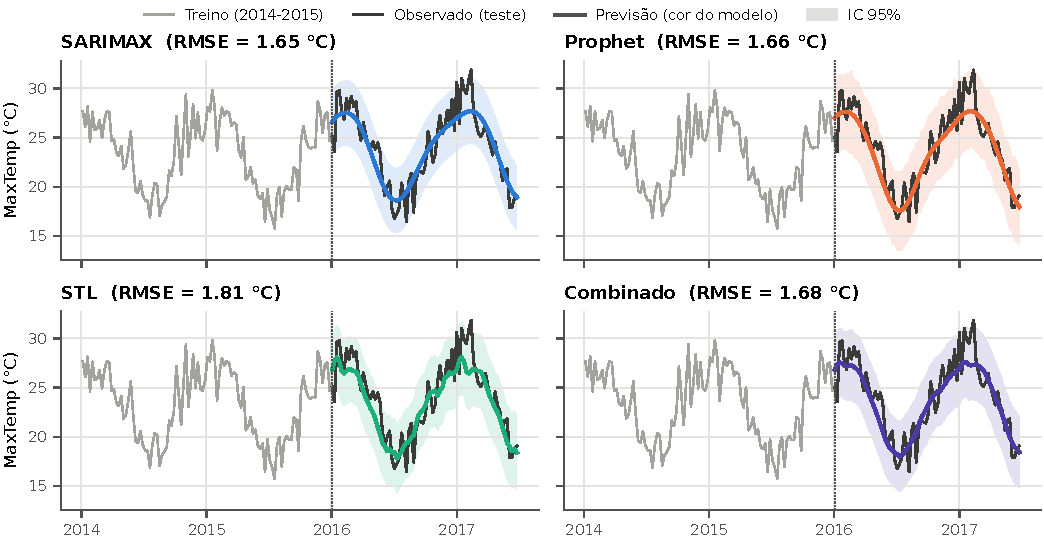
\includegraphics[width=\textwidth]{reg_previsoes.pdf}
\caption{Previsões de longo prazo (h = 1 a 78 semanas) a partir do fim de 2015, com intervalos
de 95\%. Em cinza, o final do treino; em preto, o observado no teste.}
\label{fig:prev}
\end{figure*}

\begin{figure}[!t]
\centering
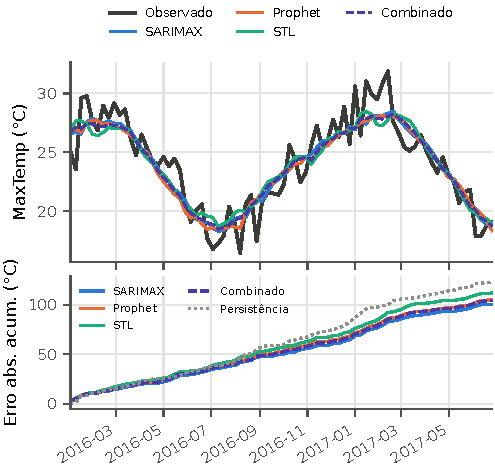
\includegraphics[width=\columnwidth]{reg_um_passo.pdf}
\caption{Cenário um passo à frente no teste. Acima: previsões contra o observado. Abaixo: erro
absoluto acumulado, em que curvas mais baixas indicam modelos melhores e a inclinação mostra
onde cada um perde, como no verão quente de 2016/17.}
\label{fig:um_passo}
\end{figure}

\begin{table}[!t]
\centering
\caption{\textit{Backtest} com origem móvel: RMSE (°C) ao prever cada ano inteiro ($h=52$), treinando só com os anos anteriores.}
\label{tab:reg_bt}
\tabfont
\resizebox{\columnwidth}{!}{\begin{tabular}{lrrrrrr}
\toprule
 & 2012 & 2013 & 2014 & 2015 & Média & DP \\
\midrule
SARIMAX & 1,36 & 1,87 & 1,86 & 1,63 & 1,68 & 0,24 \\
Prophet & 1,39 & 1,78 & 1,89 & 1,54 & \textbf{1,65} & 0,23 \\
STL & 1,76 & 1,81 & 1,97 & 1,60 & 1,78 & 0,15 \\
Combinado & 1,44 & 1,80 & 1,89 & 1,56 & 1,67 & 0,21 \\
Ingênuo sazonal & 2,69 & 2,30 & 2,57 & 2,25 & 2,45 & 0,21 \\
\bottomrule
\end{tabular}
}
\end{table}

\textbf{Significância.} O teste de Diebold--Mariano~\cite{diebold1995comparing}, com correção
de pequenas amostras~\cite{harvey1997testing} aplicada aos erros um passo à frente
(Tabela~\ref{tab:dm}), mostra que, a 5\% e sem correção para múltiplas comparações, o SARIMAX é
significativamente melhor que a persistência
($p=0{,}016$) e que a STL ($p=0{,}036$), mas não se distingue do Prophet ($p=0{,}20$) nem da
combinação ($p=0{,}16$). Com correção de Bonferroni para as quatro comparações ($\alpha=0{,}0125$),
nenhuma diferença seria significativa. O \textit{backtest} confirma esse empate técnico: as médias dos quatro
modelos ficam entre 1,65 e 1,78\,°C, contra 2,45\,°C do ingênuo, e o ranking muda de ano para
ano. O Prophet tem a menor média, e a combinação, a segunda menor, com desvio-padrão inferior ao
do SARIMAX.

\begin{table}[!t]
\centering
\caption{Teste de Diebold--Mariano: SARIMAX contra os demais modelos (erros um passo à frente). DM~$<0$ favorece o SARIMAX.}
\label{tab:dm}
\tabfont
\begin{tabular}{lrr}
\toprule
 & DM & p-valor \\
\midrule
Prophet & $-$1,298 & 0,198 \\
STL & $-$2,140 & 0,036 \\
Combinado & $-$1,410 & 0,163 \\
Persistência & $-$2,453 & 0,016 \\
\bottomrule
\end{tabular}

\end{table}

\textbf{Análise de resíduos.} A Tabela~\ref{tab:res} e a Fig.~\ref{fig:res} avaliam as
premissas usando os resíduos dentro da amostra, sem o primeiro ano. No SARIMAX, não se rejeita a média nula
($p=0{,}89$) nem se detecta autocorrelação (Ljung--Box~\cite{ljung1978measure} com 10 e 52
defasagens: $p=0{,}60$ e $0{,}26$) ou heterocedasticidade condicional
(ARCH-LM~\cite{engle1982arch}: $p=0{,}75$). A normalidade é rejeitada
(Jarque--Bera~\cite{jarque1980efficient} e Shapiro--Wilk~\cite{shapiro1965analysis}): o gráfico Q-Q mostra centro gaussiano e alguns pontos na cauda direita,
correspondentes a ondas de calor como a de fevereiro de 2011, cuja semana teve média de
34,9\,°C. Com $n=360$ semanas, os testes detectam desvios pequenos, e o efeito prático é modesto
(cobertura de 93,6\% no teste). Já os resíduos do Prophet são autocorrelacionados ($p<0{,}001$):
o modelo descreve apenas tendência e sazonalidade e deixa a persistência de curto prazo no erro.

\begin{table}[!t]
\centering
\caption{Diagnóstico dos resíduos dentro da amostra (2009--2015): média e p-valores dos testes t (média nula), Ljung--Box com 10 e 52 defasagens (LB), Jarque--Bera (JB), Shapiro--Wilk (SW) e ARCH-LM com 10 defasagens.}
\label{tab:res}
\tabfont
\resizebox{\columnwidth}{!}{\begin{tabular}{lrrrrrrr}
\toprule
 & Média & $p_t$ & LB(10) & LB(52) & JB & SW & ARCH(10) \\
\midrule
SARIMAX & 0,013 & 0,886 & 0,595 & 0,260 & 0,000 & 0,001 & 0,747 \\
Prophet & $-$0,027 & 0,761 & 0,000 & 0,000 & 0,000 & 0,002 & 0,925 \\
STL & 0,023 & 0,797 & 0,600 & 0,052 & 0,000 & 0,000 & 0,942 \\
Combinado & 0,003 & 0,976 & 0,596 & 0,162 & 0,000 & 0,000 & 0,942 \\
\bottomrule
\end{tabular}
}
\end{table}

\begin{figure*}[!t]
\centering
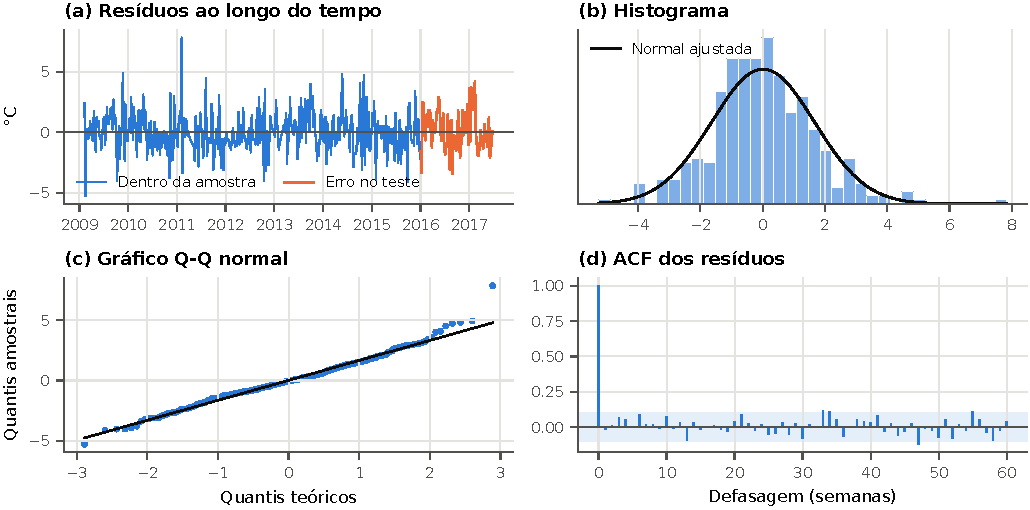
\includegraphics[width=\textwidth]{reg_residuos.pdf}
\caption{Resíduos do melhor modelo (SARIMAX). (a) Resíduos dentro da amostra (azul) e erros
de previsão no teste (laranja). (b) Histograma com a normal ajustada. (c) Gráfico Q-Q normal.
(d) ACF dos resíduos com banda de 95\%.}
\label{fig:res}
\end{figure*}

\subsection{Configuração da classificação}
Usei um \emph{holdout temporal}: treino de nov/2007 a dez/2015 (116.219 dias-estação, 22,3\%
positivos) e teste de jan/2016 a jun/2017 (25.974; 22,9\% positivos). Imputação, \textit{target
encoding} e padronização ficam dentro de um \texttt{Pipeline} do scikit-learn, reajustado em
cada dobra. Os hiperparâmetros foram buscados com 3 dobras estratificadas, maximizando a
ROC-AUC (Tabela~\ref{tab:hp_clf}). Para KNN, Random Forest e LightGBM, a busca usou uma
amostra estratificada de 40 mil linhas, por custo computacional. A robustez foi medida com
\textbf{validação cruzada estratificada de 5 dobras} no treino completo. Os pesos de classe
(\textit{balanced}) foram aplicados à logística, à Random Forest e ao LightGBM. Para cada
modelo, o limiar de decisão foi o que maximiza o F1 nas previsões \emph{fora da dobra} do
treino; só depois ele foi aplicado ao teste.

\begin{table*}[!t]
\centering
\caption{Hiperparâmetros selecionados (busca com 3 dobras, ROC-AUC).}
\label{tab:hp_clf}
\tabfont
\begin{tabular}{llrl}
\toprule
 & Melhores hiperparâmetros & AUC (busca) & Amostra \\
\midrule
Regressão Logística & C=0.1 & 0,8730 & 116 mil \\
KNN & k=61, pesos=distance & 0,8754 & 40 mil \\
Random Forest & min\_folha=1, max\_feat=0.4, prof.=None & 0,8873 & 40 mil \\
LightGBM & lambda=1.0, folhas=127, árvores=1000, min\_filhos=50, eta=0.02, colsample=0.6 & 0,8972 & 40 mil \\
\bottomrule
\end{tabular}

\end{table*}

\begin{figure*}[!t]
\centering
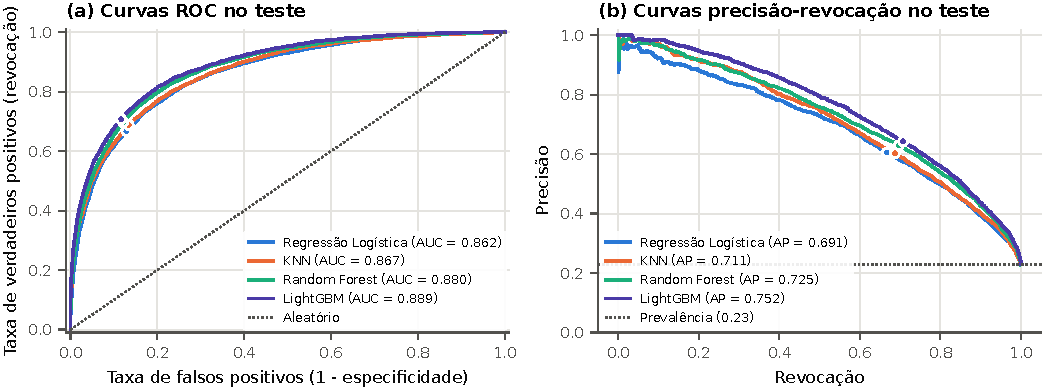
\includegraphics[width=\textwidth]{clf_roc_pr.pdf}
\caption{(a) Curvas ROC e (b) curvas precisão--revocação no conjunto de teste. Os pontos marcam
o limiar escolhido para cada modelo; as linhas pontilhadas são o classificador aleatório e a prevalência.}
\label{fig:roc}
\end{figure*}

\begin{figure*}[!t]
\centering
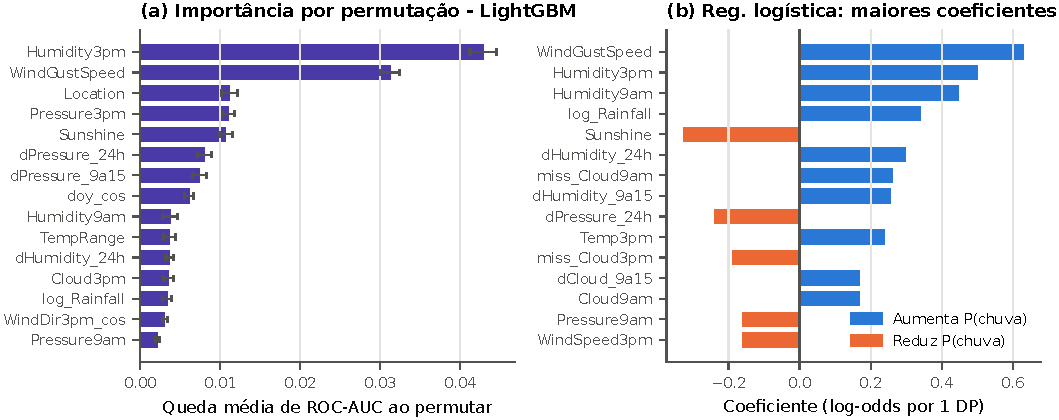
\includegraphics[width=\textwidth]{clf_importancia.pdf}
\caption{(a) Importância por permutação no teste (queda de ROC-AUC, média $\pm$ desvio em 5
repetições) do LightGBM. (b) Os 15 maiores coeficientes da regressão logística, sobre
preditores padronizados: azul aumenta e laranja reduz a probabilidade de chuva.}
\label{fig:imp}
\end{figure*}


\subsection{Resultados da classificação}

\textbf{Validação cruzada.} A variação entre dobras é pequena (desvio-padrão $\le0{,}003$ na
AUC), e o ordenamento LightGBM $>$ Random Forest $>$ KNN $>$ logística é o mesmo em todas as
dobras (Tabela~\ref{tab:cv} e Fig.~\ref{fig:cv}). Com limiar de 0,5, KNN e Random Forest têm
revocação baixa (0,46 e 0,50): o KNN não usa pesos de classe, e a Random Forest, mesmo com pesos,
concentra as probabilidades da classe minoritária abaixo de 0,5. Por isso o ajuste do limiar
(para 0,28 e 0,32, respectivamente) é essencial.

\begin{table*}[!t]
\centering
\caption{Validação cruzada estratificada de 5 dobras no treino (média $\pm$ desvio-padrão; métricas de limiar com corte em 0,5).}
\label{tab:cv}
\tabfont
\begin{tabular}{lcccccc}
\toprule
 & ROC-AUC & PR-AUC & F1 & Revocação & Precisão & Acurácia bal. \\
\midrule
Regressão Logística & 0,873 $\pm$ 0,003 & 0,702 $\pm$ 0,006 & 0,628 $\pm$ 0,004 & 0,774 $\pm$ 0,009 & 0,528 $\pm$ 0,004 & 0,788 $\pm$ 0,004 \\
KNN & 0,884 $\pm$ 0,002 & 0,728 $\pm$ 0,003 & 0,579 $\pm$ 0,003 & 0,456 $\pm$ 0,005 & 0,796 $\pm$ 0,004 & 0,711 $\pm$ 0,002 \\
Random Forest & 0,898 $\pm$ 0,002 & 0,748 $\pm$ 0,005 & 0,614 $\pm$ 0,003 & 0,503 $\pm$ 0,005 & 0,788 $\pm$ 0,007 & 0,732 $\pm$ 0,002 \\
LightGBM & 0,908 $\pm$ 0,002 & 0,776 $\pm$ 0,005 & 0,690 $\pm$ 0,005 & 0,767 $\pm$ 0,004 & 0,627 $\pm$ 0,009 & 0,818 $\pm$ 0,002 \\
\bottomrule
\end{tabular}

\end{table*}

\begin{figure}[!t]
\centering
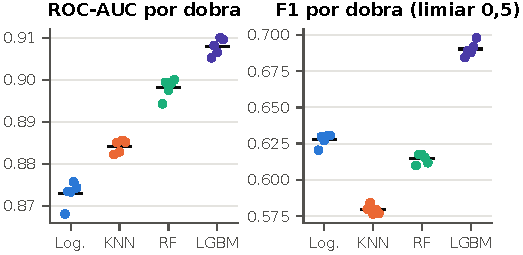
\includegraphics[width=\columnwidth]{clf_cv.pdf}
\caption{ROC-AUC e F1 em cada uma das 5 dobras; o traço preto marca a média.}
\label{fig:cv}
\end{figure}

\begin{figure}[!t]
\centering
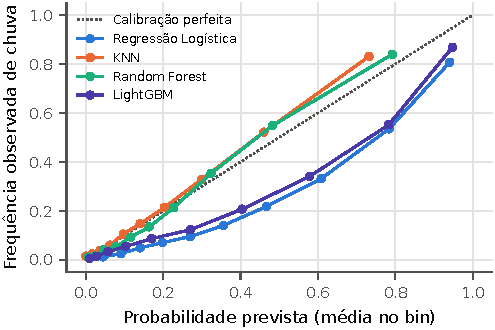
\includegraphics[width=\columnwidth]{clf_calibracao.pdf}
\caption{Curvas de confiabilidade no teste (10 \textit{bins} por quantil). Pontos abaixo da
diagonal indicam probabilidades superestimadas.}
\label{fig:calib}
\end{figure}


\textbf{Teste temporal.} O LightGBM venceu em todas as métricas de discriminação
(Tabela~\ref{tab:clf_teste}): ROC-AUC de 0,889, com IC~95\% por
\textit{bootstrap}~\cite{efron1979bootstrap} de [0,884; 0,893], PR-AUC de 0,752 e F1 de 0,674.
A Random Forest ficou em segundo lugar (AUC de 0,880 [0,875; 0,884]). Os intervalos desses dois
modelos ficam acima das AUCs da logística (0,862) e do KNN (0,867); como todos são avaliados no
mesmo teste, um teste pareado, como o de DeLong~\cite{delong1988comparing}, seria a comparação
mais rigorosa. As curvas ROC e
precisão--revocação aparecem na Fig.~\ref{fig:roc}. Sob desbalanceamento, a curva PR é mais
informativa~\cite{saito2015precision}: a linha de base é a prevalência (0,23), e a vantagem do
\textit{boosting} fica mais nítida. As AUCs de teste são 0,01--0,02 menores que as da validação
cruzada, provavelmente porque o teste está no futuro e as dobras aleatórias misturam dias vizinhos entre
treino e validação.

\begin{table}[!t]
\centering
\caption{Desempenho no teste temporal (2016--2017), com limiar (Lim.) escolhido fora da dobra. Acur.: acurácia; Prec.: precisão; Rev.: revocação; AUC: área sob a curva ROC; AP: precisão média (PR-AUC); Brier: erro quadrático das probabilidades (menor é melhor).}
\label{tab:clf_teste}
\tabfont
\resizebox{\columnwidth}{!}{\begin{tabular}{lrrrrrrrr}
\toprule
 & Lim. & Acur. & Prec. & Rev. & F1 & AUC & AP & Brier \\
\midrule
Logística & 0,604 & 0,824 & 0,606 & 0,668 & 0,635 & 0,862 & 0,691 & 0,147 \\
KNN & 0,282 & 0,825 & 0,603 & 0,688 & 0,642 & 0,867 & 0,711 & 0,113 \\
Random Forest & 0,317 & 0,837 & 0,630 & 0,697 & 0,662 & 0,880 & 0,725 & \textbf{0,108} \\
LightGBM & 0,571 & \textbf{0,843} & \textbf{0,643} & \textbf{0,708} & \textbf{0,674} & \textbf{0,889} & \textbf{0,752} & 0,122 \\
\bottomrule
\end{tabular}
}
\end{table}


\textbf{Matriz de confusão.} Com o limiar ótimo de 0,57, o LightGBM identifica 4.207 dos
5.946 dias com chuva (revocação de 70,8\%), acerta 64,3\% das vezes em que prevê chuva
(precisão) e classifica corretamente 88,3\% dos dias secos (Fig.~\ref{fig:cm}). O limiar é uma
decisão de custo: com 0,50, a revocação sobe para 76,0\%, ao preço de 705 alarmes falsos a mais.

\begin{figure}[!t]
\centering
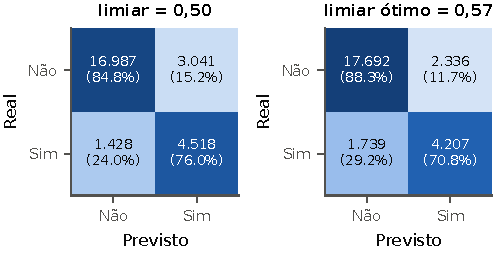
\includegraphics[width=\columnwidth]{clf_confusao.pdf}
\caption{Matriz de confusão do LightGBM no teste: contagens e percentuais por classe real, com
limiar de 0,50 (esquerda) e com o limiar que maximiza o F1 fora da dobra (direita).}
\label{fig:cm}
\end{figure}

\textbf{Interpretação.} A importância por permutação~\cite{breiman2001rf} do LightGBM e os coeficientes
padronizados da logística (Fig.~\ref{fig:imp}) concordam no topo: \texttt{Humidity3pm} e
\texttt{WindGustSpeed} dominam, como esperado fisicamente, pois ar úmido à tarde e rajadas
fortes acompanham a chegada de sistemas frontais; ambas, além disso, são medidas dentro da
janela do alvo (Seção~\ref{sec:metodo}). No LightGBM seguem a estação (\texttt{Location}), a
pressão das 15h, a insolação e duas tendências barométricas criadas na engenharia de atributos,
\texttt{dPressure\_24h} e \texttt{dPressure\_9a15}. Na logística, \texttt{dPressure\_24h} tem
coeficiente negativo: pressão em queda aumenta a chance de chuva. Como a permutação subestima
variáveis correlacionadas entre si (por exemplo, \texttt{Humidity3pm} e
\texttt{dHumidity\_9a15}), esse ranking é indicativo.
Na logística, um desvio-padrão a mais de rajada multiplica a chance de chuva por 1,88, e um a
mais de umidade às 15h, por 1,65.


\textbf{Calibração.} A logística e o LightGBM, treinados com pesos de classe,
superestimam a probabilidade de chuva (Fig.~\ref{fig:calib}), efeito esperado da
reponderação. A Random Forest, embora também ponderada, fica acima da diagonal, como o KNN, ou seja, subestima a
probabilidade, pois a média dos votos das árvores comprime as probabilidades, o mesmo efeito que leva seu
limiar ótimo a 0,32. Isso não afeta a AUC nem o F1 com limiar ajustado, mas explica por que o escore
de Brier~\cite{brier1950verification} do LightGBM (0,122) é pior que o da Random Forest (0,108).


% ===========================================================================
\section{Discussão e conclusão}\label{sec:disc}

\textbf{Regressão.} O SARIMAX com harmônicos e erros ARMA foi o melhor modelo no teste por
três motivos: (i) a série é dominada por uma sazonalidade suave, que dois harmônicos descrevem
com poucos parâmetros; (ii) os erros ARMA absorvem a persistência de curto prazo e deixam
resíduos sem autocorrelação detectável, o que rende ganho no cenário de um passo à frente; e (iii) a estimação por
máxima verossimilhança, com seleção pelo AIC, controla a complexidade. Prophet e SARIMAX
convergem para a mesma ``climatologia'' no longo prazo, e as diferenças entre eles não são
estatisticamente significativas. A STL foi prejudicada pelo perfil sazonal estimado semana a
semana, mais ruidoso, e pelo índice $c = t \bmod 52$: com período de 52,18 semanas, a fase
do perfil desliza cerca de uma semana a cada 5,6 anos. A combinação não superou o melhor modelo porque os erros dos componentes
são muito correlacionados (todos erram juntos nas ondas de calor), mas foi a segunda opção mais
estável no \textit{backtest}. Na prática, ela continua sendo uma escolha defensiva sensata
quando não se sabe de antemão qual modelo vencerá.

\textbf{Classificação.} Os \textit{ensembles} de árvores superaram os modelos linear e baseado
em distância porque capturam interações (por exemplo, umidade alta \emph{e} pressão em queda) e
não linearidades sem especificação manual. O \textit{boosting}, ao corrigir sequencialmente os
erros, foi o mais eficiente. A logística, embora inferior, continua valiosa pela
interpretabilidade e confirma a física do problema.

\textbf{Limitações.} (i) A regressão usa uma única estação e nenhuma covariável climática de
grande escala (por exemplo, ENSO/SOI), que poderiam melhorar o longo prazo. (ii) A cauda
direita dos resíduos não é gaussiana, o que sugere intervalos por \textit{bootstrap} ou erros
t-Student. (iii) A validação cruzada com dobras aleatórias, usada também na busca de hiperparâmetros
e na escolha do limiar, é levemente otimista; validação por blocos temporais ou agrupada por
data seria mais fiel. O mesmo vale para o \textit{bootstrap} dos intervalos de AUC, que trata
como independentes os dias-estação de uma mesma data. (iv) As probabilidades do LightGBM
precisam de calibração (Platt~\cite{platt1999probabilistic} ou
isotônica~\cite{zadrozny2002transforming}). (v) Parte dos preditores é medida dentro da janela
do alvo, o que torna a tarefa em parte \textit{nowcasting}. (vi) Os dados terminam em 2017.

\textbf{Pronto para produção?} Os dois modelos vencedores são reprodutíveis, rápidos e
superam com folga as referências. Antes de uso operacional, porém, seria preciso retreiná-los
com dados recentes do BoM, calibrar as probabilidades, definir o limiar a partir de uma matriz
de custos real e monitorar a deriva causada pelas mudanças climáticas. Como prova de conceito,
os resultados são sólidos; como sistema de alerta, ainda precisam dessas melhorias.

% ===========================================================================
\bibliographystyle{IEEEtran}
\bibliography{references}

\end{document}
